
\begin{dsaCharacterSheet}

\renewcommand{\arraystretch}{1}
 \setlength{\tabcolsep}{1pt}

\vspace*{-13pt}
\begin{dsaSheetBox}[\textwidth]
    \directlua{common.value_line:render({"AT", "PA", "FK", "eGS"}, "32pt")}
\end{dsaSheetBox}

\vspace{-16pt}
\dsaHeading{Waffen \& Kampfwerte}
\vspace{-8pt}

\renewcommand{\arraystretch}{1}
\setlength{\tabcolsep}{1pt}
\normalfont\fontsize{8}{12}\selectfont

\newcommand{\dsaTSHeading}[1]{\normalfont\bfseries\scriptsize #1}

\newcommand{\RS}[1]{%
    \makebox(.7cm,.8em)[c]{\normalfont\directlua{kampfbogen.ruestung("#1")}  \hspace{-2.5pt}}
}

\begin{dsaSheetBox}[\textwidth]
    \begin{NiceTabular}{p{4.8cm}|x{1.8cm}@{/}x{0.5cm}|x{1cm}|x{1.4cm}|x{0.8cm}@{/}x{0.7cm}|x{1cm}|x{0.6cm}@{/}x{0.6cm}|x{0.8cm}|x{0.8cm}|x{1.4cm}|x{0.5cm}|x{0.5cm}}
    \CodeBefore\rowcolors{2}{white}{gray!30}\Body
        \dsaTHeading{Nahkampfwaffe} &
        \multicolumn{2}{c|}{\dsaTHeading{Typ/eBE}} &
        \dsaTHeading{DK} &
        \dsaTHeading{TP} &
        \multicolumn{2}{c|}{\dsaTHeading{TP/KK}} &
        \dsaTHeading{INI} &
        \multicolumn{2}{c|}{\dsaTHeading{WM}} &
        \dsaTHeading{AT} &
        \dsaTHeading{PA} &
        \dsaTHeading{TP} &
        \multicolumn{2}{c}{\dsaTHeading{BF}} \\ \Xhline{2\arrayrulewidth}
        \directlua{
            kampfbogen.nahkampf()
        } \\ \Xhline{3\arrayrulewidth}
    \end{NiceTabular}

    \vspace{2pt}
    \begin{tabular}{p{\textwidth-1.33\tabcolsep}}
        \directlua{
            common.multiline_content({
                name="Nahkampf-SF", rows=common.current_page.Nahkampf.SF,
                preamble="\noexpand\\footnotesize Sonderfertigkeiten",
                baselinestretch=1.04, hspace="5pt", fontsize={8,12}
            }, data.SF.Nahkampf)
        }
    \end{tabular}
\end{dsaSheetBox}

\begin{dsaSheetBox}[\textwidth]
    \begin{NiceTabular}{p{4.5cm}|x{1.65cm}@{/}x{0.5cm}|x{1.4cm}|x{0.6cm}@{/}x{0.6cm}@{/}x{0.6cm}@{/}x{0.6cm}@{/}x{0.6cm}|x{0.6cm}@{/}x{0.6cm}@{/}x{0.6cm}@{/}x{0.6cm}@{/}x{0.6cm}|x{0.8cm}|x{1.2cm}|x{0.7cm}}
    \CodeBefore\rowcolors{2}{white}{gray!30}\Body
        \dsaTHeading{Fernkampfwaffe} &
        \multicolumn{2}{c|}{\dsaTHeading{Typ/eBE}} &
        \dsaTHeading{TP} &
        \multicolumn{5}{c|}{\dsaTHeading{Entfernungen}} &
        \multicolumn{5}{c|}{\dsaTHeading{TP/Entfernung}} &
        \dsaTHeading{FK} &
        \dsaTHeading{Laden} &
        \hspace{-2pt}\raisebox{-2pt}{
            \def\arrow{
                (2,0) -- (2,2) -- (0,2) -- (2, 4) -- (3, 4) -- (6, 7) -- (5, 8) -- (9, 9) -- (8, 5) -- (7, 6) -- (4, 3) -- (4, 2) -- cycle
            }
            \begin{tikzpicture}[scale=0.04]
                \begin{scope}[rotate=-30]
                    \path[fill=gray, shift={(1.5, -1.25)}] \arrow;
                    \path[fill=black] \arrow;
                \end{scope}
            \end{tikzpicture}
        } \\ \Xhline{2\arrayrulewidth}
        \directlua{
            kampfbogen.fernkampf()
        } \\ \Xhline{3\arrayrulewidth}
    \end{NiceTabular}

    \vspace{2pt}
    \begin{tabular}{p{\textwidth-1.33\tabcolsep}}
        \directlua{
            common.multiline_content({
                name="Fernkampf-SF", rows=common.current_page.Fernkampf.SF,
                preamble="\noexpand\\footnotesize Sonderfertigkeiten",
                baselinestretch=1.04, hspace="5pt", fontsize={8,12}
            }, data.SF.Fernkampf)
        }
    \end{tabular}
\end{dsaSheetBox}

\begin{minipage}{12.6cm}
	\begin{dsaSheetBox}[\textwidth]
        \begin{NiceTabular}{p{4.85cm}|x{0.6cm}@{/}x{0.6cm}|x{1cm}|x{1cm}|x{1cm}|x{2.5cm}}
        \CodeBefore\rowcolors{2}{white}{gray!30}\Body
            \dsaTHeading{Waffenloser Kampf} &
            \multicolumn{2}{c|}{\dsaTHeading{TP/KK}} &
            \dsaTHeading{INI} &
            \dsaTHeading{AT} &
            \dsaTHeading{PA} &
            \dsaTHeading{TP(A)} \\ \Xhline{2\arrayrulewidth}
            \directlua{
                kampfbogen.waffenlos()
            } \\ \Xhline{3\arrayrulewidth}
        \end{NiceTabular}

        \vspace{2pt}
        \begin{tabular}{p{\textwidth-1.33\tabcolsep}}
            \directlua{
                common.multiline_content({
                  name="Waffenlos-SF", rows=common.current_page.Waffenlos.SF,
                  preamble="\noexpand\\footnotesize Sonderfertigkeiten",
                  baselinestretch=1.04, hspace="5pt", fontsize={8,12}
                }, data.SF.Waffenlos)
            }
        \end{tabular}
    \end{dsaSheetBox}
	\vspace{-28pt}
    \begin{center}
        \LARGE\bfseries\textmansontt{\shadowtext{Schild / Parierwaffe}}%
    \end{center}%
    \vspace{-4pt}

    \begin{dsaSheetBox}
        \begin{NiceTabular}{p{4.85cm}|x{2.6cm}|x{1cm}|x{0.6cm}@{/}x{0.6cm}|x{0.8cm}|x{0.5cm}|x{0.5cm}}
        \CodeBefore\rowcolors{2}{white}{gray!30}\Body
            \dsaTHeading{Name} &
            \dsaTHeading{Typ} &
            \dsaTHeading{INI} &
            \multicolumn{2}{c|}{\dsaTHeading{WM}} &
            \dsaTHeading{PA} &
            \multicolumn{2}{c}{\dsaTHeading{BF}} \\ \Xhline{2\arrayrulewidth}
            \directlua{
                kampfbogen.schilde()
            } \\ \Xhline{3\arrayrulewidth}%
        \end{NiceTabular}

        \vspace{2pt}
        \footnotesize\normalfont\bfseries\centering
        \directlua{
            common.checkboxlist({
                {"Linkhand (PA+1)", data.SF.Nahkampf.Linkhand},
                {{"Schildkampf I (PA+2)", "II (PA+2)"},
                    data.SF.Nahkampf:getlist("Schildkampf")},
                {{"Parierwaffen I", "II"}, data.SF.Nahkampf:getlist("Parierwaffen")}
            })
        }
    \end{dsaSheetBox}

	\vspace{4pt}
	\begin{minipage}{6cm}
		\begin{center}
            \LARGE\bfseries\textmansontt{\shadowtext{Rüstung}}%
        \end{center}%
        \vspace{-4pt}

        \begin{dsaSheetBox}
            \begin{NiceTabular}{p{3.8cm}|x{0.8cm}|x{0.8cm}}
            \CodeBefore
                \rowcolors{2-7}{white}{gray!30}
                \cellcolor{gray!30}{8-2,8-3}
                \cellcolor{white}{9-3}
            \Body
                \dsaTHeading{Rüstungsstück} &
                \dsaTHeading{RS} &
                \dsaTHeading{BE} \\ \Xhline{2\arrayrulewidth}
                \directlua{
                    kampfbogen.ruestungsteile()
                } \\ \Xhline{2\arrayrulewidth}
                \normalfont\bfseries\scriptsize Summe &
                \directlua{tex.sprint(data:cur("RS"))} & \directlua{tex.sprint(data:cur("BE_voll"))} \\ \Xhline{2\arrayrulewidth}
                \multicolumn{2}{l|}{
                    \normalfont\scriptsize\bfseries Rüstungsgewöhnung
                    \directlua{
                        common.checkboxlist({
                            {{"I", "II", "III"}, data.SF.Nahkampf:getlist("Ruestungsgewoehnung")}
                        })
                    }

                } & \directlua{tex.sprint(-2, data:cur("BE"))}
            \end{NiceTabular}
        \end{dsaSheetBox}
	\end{minipage}
	\begin{minipage}{6.5cm}
		\begin{center}
            \LARGE\bfseries\textmansontt{\shadowtext{Ausweichen}}%
        \end{center}%
        \vspace{-3.5pt}

        \begin{dsaSheetBox}
            \setlength{\tabcolsep}{0pt}
            \tiny\normalfont\bfseries
            \begin{tabular}{x{1cm}p{0.3cm}x{0.7cm}p{0.3cm}x{2.5cm}p{0.3cm}x{1cm}}
                \multicolumn{2}{l}{\scriptsize PA-Basis} & \scriptsize BE & & \scriptsize SF Ausweichen & & \scriptsize Summe \\
                \normalsize \directlua{tex.sprint(-2, data:cur("PA"))} &
                \normalsize $-$ &
                \normalsize \directlua{tex.sprint(-2, data:cur("BE"))} &
                \normalsize $+$ &
                \begin{minipage}{2.5cm}
                    \centering
                    \directlua{common.checkboxlist({{{"I", "II", "III"}, data.SF.Nahkampf:getlist("Ausweichen")}})} \\
                    jeweils +3 \\
                    Flink (+1) / Behäbig (-1)?
                \end{minipage}
                & \normalsize $=$ &
                \normalsize \directlua{kampfbogen.ausweichen()}
                \\ \Xcline{1-1}{3\arrayrulewidth} \Xcline{3-3}{3\arrayrulewidth} \Xcline{7-7}{3\arrayrulewidth}
                 & & & \multicolumn{3}{c}{Akrobatik (+$\lfloor(\mathrm{TaW}-9) / 3 \rfloor $)?} &
            \end{tabular}
        \end{dsaSheetBox}

		\vspace{-4.8pt}
		\begin{center}
            \LARGE\bfseries\textmansontt{\shadowtext{Wunden}}%
        \end{center}%
        \vspace{-3pt}

        \begin{dsaSheetBox}
            \centering
            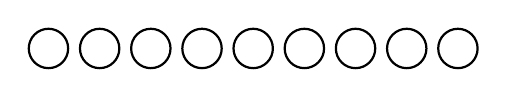
\begin{tikzpicture}
                \filldraw[fill=white, draw=black, thick] (1,1) circle (0.25cm);
                \filldraw[fill=white, draw=black, thick] (1.65,1) circle (0.25cm);
                \filldraw[fill=white, draw=black, thick] (2.3,1) circle (0.25cm);
                \filldraw[fill=white, draw=black, thick] (2.95,1) circle (0.25cm);
                \filldraw[fill=white, draw=black, thick] (3.6,1) circle (0.25cm);
                \filldraw[fill=white, draw=black, thick] (4.25,1) circle (0.25cm);
                \filldraw[fill=white, draw=black, thick] (4.9,1) circle (0.25cm);
                \filldraw[fill=white, draw=black, thick] (5.55,1) circle (0.25cm);
                \filldraw[fill=white, draw=black, thick] (6.2,1) circle (0.25cm);
            \end{tikzpicture} \\
            \scriptsize\normalfont\bfseries je Wunde AT, PA, FK, GE, INI - 2, GS - 1
        \end{dsaSheetBox}
	\end{minipage}
\end{minipage}
\begin{minipage}{\textwidth-12.6cm-\fboxsep}
    \normalfont\bfseries
    \directlua{kampfbogen.silhouette()}
\end{minipage}

\vspace{-10pt}
\begin{center}%
    \LARGE\bfseries\textmansontt{\shadowtext{Lebensenergie, Ausdauer, etc.}}%
\end{center}%
\vspace{-12pt}

\begin{dsaSheetBox}
    \begin{NiceTabular}{p{3cm}|x{1cm}|x{1cm}|x{1cm}|x{1cm}|p{11.1cm}}
    \CodeBefore\rowcolors{2}{white}{gray!30}\Body
        & \dsaTSHeading{max.} & \dsaTSHeading{1/2} & \dsaTSHeading{1/3} & \dsaTSHeading{1/4} & \normalfont\bfseries\scriptsize\hspace{2pt} aktuell \\ \Xhline{2\arrayrulewidth}
        \directlua{kampfbogen.energieleiste("Lebensenergie", data:cur("LE"))} \\ \hline
        \directlua{kampfbogen.energieleiste("Ausdauer", data:cur("AU"))}
        \directlua{kampfbogen.optionalleiste("Astralenergie", data:cur("AE"))}
        \directlua{kampfbogen.optionalleiste("Karmaenergie", data:cur("KE"))}
    \end{NiceTabular}
\end{dsaSheetBox}

\begin{dsaSheetBox}
    \vspace*{-4pt}
    \large{}
    \setlength\fboxsep{3pt}
    \parbox{3cm}{\bfseries\textmansontt{Initiative:}}
    \colorbox{white}{\parbox[c]{15.4cm}{\directlua{kampfbogen.ini()}}}
    
    \vspace*{-0pt}
\end{dsaSheetBox}

\end{dsaCharacterSheet}